\chapter{Linearization Method}\label{chap:content}

Though this will not always be possible, we want to impose a total order on the task networks, such that for a method $m = (c, (T, \singlePrec, \alpha))$, the decomposition of $t$ will result in an executable sequence. To attempt this, one could analyse what preconditions the execution of sub-tasks in $T$ might need, and what effects they might have. 


For example, if a sub-task $t$ deletes a fact in the precondition for sub-task $t'$, one could order $t'$ before $t$ to avoid invalidating the precondition for $t'$. So we need a way of estimating preconditions and effects for compound tasks. It was proven by \cite{ConnyPreEstimation} that inferring all preconditions and effects of a compound task is as difficult as solving the problem. Therefore, a polynomial-time algorithm to infer the \textit{exact} set of preconditions and effects of a compound task does not exist. 

However, using an approximated set, one can analyse the proposed orderings and resolve any conflicts, e.g. cycles. If conflict-resolution is necessary, we refer to this as needing \textbf{\textit{cycle-breaking}}.

The algorithm provided in this paper approximates possible preconditions and effects for all tasks so that this information can be used to linearize methods. 
For a given task $t$, we  call these approximate preconditions and effects as $\PreS(t), \DelS(t), \AddS(t)$.
If t is an action, $\PreS(t), \DelS(t), \AddS(t)$ is the same as $\Pre(t), \Add(t), \Del(t)$. 
If t is a compound task, $\PreS(t)$, $\AddS(t),  \DelS(t)$, are the union of the respective preconditions, add, and delete effects of all actions that $t$ could decompose to, as shown in Figure~\ref{CompoundPreEff} and \ref{CompoundPreEffForLifted}.
This means that for a task $t$ $\PreS(t), \DelS(t), \AddS(t)$ can contain contradictory effects, e.g. $t$ adds \emph{and} deletes a fact. These are essentially the mentioned literals defined by \cite{mentionedliterals}.

\newpage
\begin{figure}[h]
	\begin{subfigure}{4.5cm}  \caption{Example of a ground task network}
		\scalebox{0.7} {
			\begin{tikzpicture}[->,auto,node distance=1.2cm,
			thick,main node/.style={circle,draw,font=\sffamily\Large\bfseries},
			square effect/.style={rectangle,draw,font=\sffamily\Large\bfseries}]
			
						\action{1}{SubTaskC,
				width  = 2.5em, 
				height = 2.5em,
				pre length = 2em,
				eff length = 2em,
				body = {rounded corners} 
			}			
			\action{2}{SubTaskD,
				width  = 2.5em, 
				height = 2.5em, 
				body = {rounded corners, below = 1em of 1} 
			}		
		
			\action{3}{PrimitiveE,
			width  = 1.2em, 
			height = 1.2em,
			eff length = 2em,
			body = {below left = 2em and 3.5em of 1}
			}
			
			\action{4}{PrimitiveF,
				width  = 1.2em, 
				height = 1.2em,
				eff length = 2em,
				body = {below left = 2em and 3em of 2}
			}	
			
			\action{5}{PrimitiveG,
				width  = 1.2em, 
				height = 1.2em,
				eff length = 2em,
				body = {below right = 2em and 3em of 2}
			}
			
			\path[every node/.style={font=\sffamily\small}]
			(1) edge node [right] {} (2)
			(1) edge node [right] {} (3)
			(2) edge node [right] {} (4)	
			(2) edge node [right] {} (5);
			\end{tikzpicture}
		}
	\end{subfigure}	
	\hspace{1cm}
	\begin{subfigure}{4.5cm}  \caption{Predicates collected}
		\scalebox{0.7}{
			\begin{tikzpicture}[->,auto,node distance=1.2cm,
			thick,main node/.style={circle,draw,font=\sffamily\Large\bfseries},
			square effect/.style={rectangle,draw,font=\sffamily\Large\bfseries}]
			
						\action{1}{SubTaskC,
				width  = 2.5em, 
				height = 2.5em,
				pre length = 2em,
				eff length = 2em,
				body = {rounded corners} 
			}			
			\action{2}{SubTaskD,
				width  = 2.5em, 
				height = 2.5em, 
				body = {rounded corners, below = 1em of 1} 
			}		
		
			\action{3}{PrimitiveE,
			width  = 1.2em, 
			height = 1.2em,
			eff length = 2em,
			body = {below left = 2em and 3.5em of 1}
			}
			
			\action{4}{PrimitiveF,
				width  = 1.2em, 
				height = 1.2em,
				eff length = 2em,
				body = {below left = 2em and 3em of 2}
			}	
			
			\action{5}{PrimitiveG,
				width  = 1.2em, 
				height = 1.2em,
				eff length = 2em,
				body = {below right = 2em and 3em of 2}
			}
			\path[every node/.style={font=\sffamily\small}]
			(1) edge node [right] {} (2)
			(1) edge node [right] {} (3)
			(2) edge node [right] {} (4)	
			(2) edge node [right] {} (5);
			\end{tikzpicture}   
		}
	\end{subfigure} 
	\caption{Inferring preconditions and effects for compound tasks in grounded format}
	\label{CompoundPreEff}
\end{figure}

\vspace{1em}
\begin{figure}[h]
	\begin{subfigure}{15cm} \caption{Lifted Method Definition}
		\centering
		\scalebox{0.7} {
			\begin{tikzpicture}[->,auto,node distance=1.2cm,
			thick,main node/.style={circle,draw,font=\sffamily\Large\bfseries},
			square effect/.style={rectangle,draw,font=\sffamily\Large\bfseries}]
			
			\action{1}{CollectSoil1={rover}{pt},
				width  = 2.5em, 
				height = 2em, 
				pre length = 8em,
				eff length = 8em,
				body = {rounded corners} 
			}
			
			\action{2}{CollectSoilNavigate={pt0}{pt}{rover},
				width  = 2.5em, 
				height = 2.5em, 
				pre length = 0em,
				eff length = 0em,
				body = {below left = 2em and 1em of 1} 
			}
			
			\action{3}{CollectSoilGetSoil = {pt},
				width  = 1.2em, 
				height = 1.2em,
				pre length = 0em,
				eff length = 0em,
				body = {below right = 2em and 1em of 1}
			}
			\path[every node/.style={font=\sffamily\small}]
			(1) edge node [right] {} (2)
			(1) edge node [right] {} (3);
			\end{tikzpicture}
		}
	\end{subfigure}
	
	\vspace{1em}
	\begin{subfigure}{15cm} \caption{Lifted Action Defintion}
		\scalebox{0.7} {
			\begin{tikzpicture} 	
			[->,auto,node distance=1.2cm,
			thick,main node/.style={circle,draw,font=\sffamily\Large\bfseries},
			square effect/.style={rectangle,draw,font=\sffamily\Large\bfseries}]
			
			\action{Nav}{CollectSoilNavigate={from}{to}{rover},
				width  = 2.5em, 
				height = 2.5em, 
				pre length = 8em,
				eff length = 8em,
				body = {below = 2em of 2} 
			}
			
			\action{GetSoil}{CollectSoilGetSoil = {pt},
				width  = 1.2em, 
				height = 1.2em,
				pre length = 8em,
				eff length = 8em,
				body = {below = 3em of 3}
			}
			\end{tikzpicture}
		}
	\end{subfigure}
	
	\vspace{1em}
	\begin{subfigure}{15cm} \caption{Example of psuedo-grounded task network}
		\scalebox{0.7} {
			\begin{tikzpicture}[->,auto,node distance=1.2cm,
			thick,main node/.style={circle,draw,font=\sffamily\Large\bfseries},
			square effect/.style={rectangle,draw,font=\sffamily\Large\bfseries}]
			
			\action{1}{CollectSoil1={rover1}{pt1},
				width  = 2.5em, 
				height = 2em, 
				pre length = 8em,
				eff length = 8em,
				body = {rounded corners} 
			}
			
			\action{2}{CollectSoilNavigate={pt0}{pt1}{rover1},
				width  = 2.5em, 
				height = 2.5em, 
				pre length = 8em,
				eff length = 8em,
				body = {below left = 2em and 1em of 1} 
			}
			
			\action{3}{CollectSoilGetSoil = {pt1},
				width  = 1.2em, 
				height = 1.2em,
				pre length = 8em,
				eff length = 8em,
				body = {below right = 2em and 1em of 1}
			}
			
			\path[every node/.style={font=\sffamily\small}]
			(1) edge node [right] {} (2)
			(1) edge node [right] {} (3);
			\end{tikzpicture}
		}
	\end{subfigure}
	
	\vspace{2em}
	\begin{subfigure}{14cm} \caption{Resulting \enquote{predicates} collected}
		\centering
		\scalebox{0.7} {
			\begin{tikzpicture}[->,auto,node distance=1.2cm,
			thick,main node/.style={circle,draw,font=\sffamily\Large\bfseries},
			square effect/.style={rectangle,draw,font=\sffamily\Large\bfseries}]
			
			\action{Other}{CollectSoil2={rover}{pt},
				width  = 2em, 
				height = 4em, 
				pre length = 8em,
				eff length = 8em,
				body = {rounded corners, below = 10em of 1} 
			}
			
			\end{tikzpicture}
		}
	\end{subfigure}
	\caption{Inferring preconditions and effects for tasks in lifted format}
	\label{CompoundPreEffForLifted}
\end{figure}

\newpage
This method can be used for both lifted and grounded models. For a grounded format, collect actual predicates from the actions.
In a lifted format, tasks and methods accept parameters, referring to any object of a specific type. Thus actions have \enquote{different} but symmetrical effects and preconditions in a ground depending on actual objects passed in.
For each method, we can \enquote{ground} it in the standard way using an arbitrary object,
and the resulting \enquote{predicates} can be used to order the sub-tasks, while groundings are discarded. Where a task accepts two parameters of the same type under different names, it is assumed those are different objects, like for \enquote{Navigate(pt0, pt, rover)} sub-task in Figure~\ref{CompoundPreEffForLifted}.


Given the inferred preconditions and effects of compound tasks, when the same state variable $b$ is added by $t$,  and required by $t'$, then order $t$ before $t'$. When $b$ is added by $t$,  and deleted by $t'$, then order $t'$ before $t$. When $b$ is deleted by $t$, and required by $t'$, then order $t'$ before $t$. Figure~\ref{AddOrderings} also shows how the additional orderings for a method are determined. We then attempt to integrate these orderings into the method $m = (t, (T, \singlePrec, \alpha))$. 

If there exists a cycle after integrating the new orderings into $\singlePrec$, we remove a random one of the new orderings in that cycle, as shown in Figure~\ref{CycleBreak}, until that cycle no longer exists.
We repeat this for all methods in order to linearize them.


\begin{figure}[h]
	\scalebox{0.7}{
		\begin{subfigure}{5cm} 
			\begin{tikzpicture}[->,auto,node distance=1.2cm,
			thick,main node/.style={circle,draw,font=\sffamily\Large\bfseries},
			square effect/.style={rectangle,draw,font=\sffamily\Large\bfseries}]		
			
			\action{3}{SubTaskC,
width  = 2.5em, 
height = 2.5em, 
pre length = 2em,
eff length = 2em,
body = {rounded corners} 
}				

\action{2}{SubTaskB,
	width  = 2.5em, 
	height = 2.5em, 
	pre length = 2em,
	eff length = 2em,
	body = {rounded corners, below right = 2em and 2em of 3} 
}	

\action{1}{SubTaskA,
	width  = 2.5em, 
	height = 2.5em, 
	pre length = 2em,
	eff length = 2em,
	body = {rounded corners, above right = 2em and 2em of 2} 
}	
			
			\path[every node/.style={font=\sffamily\small}]
			(3) edge node [left]  {} (1);
			\end{tikzpicture}
			\caption{The original method}
		\end{subfigure}
	}
	\hspace{1cm}	
	\scalebox{0.7}{
		\begin{subfigure}{5cm}
			\begin{tikzpicture}[->,auto,node distance=1.2cm,
			thick,main node/.style={circle,draw,font=\sffamily\Large\bfseries},
			square effect/.style={rectangle,draw,font=\sffamily\Large\bfseries}]
			
			\action{3}{SubTaskC,
width  = 2.5em, 
height = 2.5em, 
pre length = 2em,
eff length = 2em,
body = {rounded corners} 
}				

\action{2}{SubTaskB,
	width  = 2.5em, 
	height = 2.5em, 
	pre length = 2em,
	eff length = 2em,
	body = {rounded corners, below right = 2em and 2em of 3} 
}	

\action{1}{SubTaskA,
	width  = 2.5em, 
	height = 2.5em, 
	pre length = 2em,
	eff length = 2em,
	body = {rounded corners, above right = 2em and 2em of 2} 
}
			
			\path[every node/.style={font=\sffamily\small}]
			(1) edge[dashed, bend right] node [left] {} (3)
			(3) edge node [left] {} (1);
			\end{tikzpicture}
			\caption{C deletes fact (a) in preconditions of A  -- so A before C}
		\end{subfigure}
	}
	
	\vspace{2em}
	
	\scalebox{0.7}{
		\begin{subfigure}{5cm}
			\begin{tikzpicture}[->,auto,node distance=1.2cm,
			thick,main node/.style={circle,draw,font=\sffamily\Large\bfseries},
			square effect/.style={rectangle,draw,font=\sffamily\Large\bfseries}]
			
			\action{3}{SubTaskC,
width  = 2.5em, 
height = 2.5em, 
pre length = 2em,
eff length = 2em,
body = {rounded corners} 
}				

\action{2}{SubTaskB,
	width  = 2.5em, 
	height = 2.5em, 
	pre length = 2em,
	eff length = 2em,
	body = {rounded corners, below right = 2em and 2em of 3} 
}	

\action{1}{SubTaskA,
	width  = 2.5em, 
	height = 2.5em, 
	pre length = 2em,
	eff length = 2em,
	body = {rounded corners, above right = 2em and 2em of 2} 
}
			
			\path[every node/.style={font=\sffamily\small}]
			(3) edge[dashed] node [right] {} (2)
			(1) edge[dashed, bend right] node [left] {} (3)
			(3) edge node [left] {} (1);
			\end{tikzpicture}
			\caption{B adds a fact (a) that C deletes -- so C before B}
		\end{subfigure}
	}
	\hspace{1cm}
	\scalebox{0.7}{
		\begin{subfigure}{5cm}
			\begin{tikzpicture}[->,auto,node distance=1.2cm,
			thick,main node/.style={circle,draw,font=\sffamily\Large\bfseries},
			square effect/.style={rectangle,draw,font=\sffamily\Large\bfseries}]
			
			\action{3}{SubTaskC,
width  = 2.5em, 
height = 2.5em, 
pre length = 2em,
eff length = 2em,
body = {rounded corners} 
}				

\action{2}{SubTaskB,
	width  = 2.5em, 
	height = 2.5em, 
	pre length = 2em,
	eff length = 2em,
	body = {rounded corners, below right = 2em and 2em of 3} 
}	

\action{1}{SubTaskA,
	width  = 2.5em, 
	height = 2.5em, 
	pre length = 2em,
	eff length = 2em,
	body = {rounded corners, above right = 2em and 2em of 2} 
}
			
			\path[every node/.style={font=\sffamily\small}]
			(2) edge[dashed] node [right] {} (1)
			(3) edge[dashed] node [right] {} (2)
			(1) edge[dashed, bend right] node [left] {} (3)
			(3) edge node [left] {} (1);
			\end{tikzpicture}
			\caption{B adds a fact (a) in preconditions of A -- so B before A}
		\end{subfigure}
	}
	\caption{Adding possible orderings to methods}
	
	\label{AddOrderings} 
\end{figure}



\begin{figure}
	\begin{subfigure}{5cm}
		\scalebox{1}{
			\begin{tikzpicture}[->,auto,node distance=1.5cm,
			thick,main node/.style={circle,draw,font=\sffamily\Large\bfseries},
			square effect/.style={rectangle,draw,font=\sffamily\Large\bfseries}]
			
			\action{3}{SubTaskC,
width  = 2.5em, 
height = 2.5em, 
pre length = 2em,
eff length = 2em,
body = {rounded corners} 
}				

\action{2}{SubTaskB,
	width  = 2.5em, 
	height = 2.5em, 
	pre length = 2em,
	eff length = 2em,
	body = {rounded corners, below right = 2em and 2em of 3} 
}	

\action{1}{SubTaskA,
	width  = 2.5em, 
	height = 2.5em, 
	pre length = 2em,
	eff length = 2em,
	body = {rounded corners, above right = 2em and 2em of 2} 
}
			
			\path[every node/.style={font=\sffamily\small}]
			(2) edge[dashed] node [right] {} (1)
			(3) edge[dashed] node [right] {} (2)
			(1) edge[dashed, bend right] node [left] {} (3)
			(3) edge node [left] {} (1);
			\end{tikzpicture}
		}
		\caption{Search for cycle in the modified method}
	\end{subfigure}
	\hspace{1cm}
	\begin{subfigure}{5cm}
		\scalebox{1}{
			\begin{tikzpicture}[->,auto,node distance=1.5cm,
			thick,main node/.style={circle,draw,font=\sffamily\Large\bfseries},
			square effect/.style={rectangle,draw,font=\sffamily\Large\bfseries}]
			
			\action{3}{SubTaskC,
width  = 2.5em, 
height = 2.5em, 
pre length = 2em,
eff length = 2em,
body = {rounded corners} 
}				

\action{2}{SubTaskB,
	width  = 2.5em, 
	height = 2.5em, 
	pre length = 2em,
	eff length = 2em,
	body = {rounded corners, below right = 2em and 2em of 3} 
}	

\action{1}{SubTaskA,
	width  = 2.5em, 
	height = 2.5em, 
	pre length = 2em,
	eff length = 2em,
	body = {rounded corners, above right = 2em and 2em of 2} 
}
			
			\path[every node/.style={font=\sffamily\small}]
			(2) edge[dashed] node [right] {} (1)
			(3) edge[dashed] node [right] {} (2)
			(1) edge[dashed, bend right] node [left] {} (3);
			\end{tikzpicture}
		}
		\caption{Cycle identified}
	\end{subfigure}
	
	\vspace{1em}
	\begin{subfigure}{5cm}
		\scalebox{1}{
			\begin{tikzpicture}[->,auto,node distance=1.5cm,
			thick,main node/.style={circle,draw,font=\sffamily\Large\bfseries},
			square effect/.style={rectangle,draw,font=\sffamily\Large\bfseries}]
			
			\action{3}{SubTaskC,
width  = 2.5em, 
height = 2.5em, 
pre length = 2em,
eff length = 2em,
body = {rounded corners} 
}				

\action{2}{SubTaskB,
	width  = 2.5em, 
	height = 2.5em, 
	pre length = 2em,
	eff length = 2em,
	body = {rounded corners, below right = 2em and 2em of 3} 
}	

\action{1}{SubTaskA,
	width  = 2.5em, 
	height = 2.5em, 
	pre length = 2em,
	eff length = 2em,
	body = {rounded corners, above right = 2em and 2em of 2} 
}
			
			\path[every node/.style={font=\sffamily\small}]
			%(2) edge[dashed] node [right] {} (1)
			(3) edge[dashed] node [right] {} (2)
			(1) edge[dashed, bend right] node [left] {} (3);
			\end{tikzpicture}
		}
		\caption{Pick an edge not originally in the method (i.e.\ a dashed edge) and delete it.}
		
	\end{subfigure}
	\hspace{1cm}
	\begin{subfigure}{5cm}
		\scalebox{1}{
			\begin{tikzpicture}[->,auto,node distance=1.5cm,
			thick,main node/.style={circle,draw,font=\sffamily\Large\bfseries},
			square effect/.style={rectangle,draw,font=\sffamily\Large\bfseries}]
			
			\action{3}{SubTaskC,
width  = 2.5em, 
height = 2.5em, 
pre length = 2em,
eff length = 2em,
body = {rounded corners} 
}				

\action{2}{SubTaskB,
	width  = 2.5em, 
	height = 2.5em, 
	pre length = 2em,
	eff length = 2em,
	body = {rounded corners, below right = 2em and 2em of 3} 
}	

\action{1}{SubTaskA,
	width  = 2.5em, 
	height = 2.5em, 
	pre length = 2em,
	eff length = 2em,
	body = {rounded corners, above right = 2em and 2em of 2} 
}
			
			\path[every node/.style={font=\sffamily\small}]
			%(2) edge[dashed] node [right] {} (1)
			(3) edge[dashed] node [right] {} (2)
			(1) edge[dashed, bend right] node [left] {} (3)
			(3) edge node [left] {} (1);
			\end{tikzpicture}
		}
		\caption{Repeat as necessary until depth-first search cannot find more cycles}
	\end{subfigure}
	\vspace{2cm}
	
	
	\begin{subfigure}{5cm}
		\scalebox{1}{
			\begin{tikzpicture}[->,auto,node distance=1.5cm,
			thick,main node/.style={circle,draw,font=\sffamily\Large\bfseries},
			square effect/.style={rectangle,draw,font=\sffamily\Large\bfseries}]
			
			\action{3}{SubTaskC,
width  = 2.5em, 
height = 2.5em, 
pre length = 2em,
eff length = 2em,
body = {rounded corners} 
}				

\action{2}{SubTaskB,
	width  = 2.5em, 
	height = 2.5em, 
	pre length = 2em,
	eff length = 2em,
	body = {rounded corners, below right = 2em and 2em of 3} 
}	

\action{1}{SubTaskA,
	width  = 2.5em, 
	height = 2.5em, 
	pre length = 2em,
	eff length = 2em,
	body = {rounded corners, above right = 2em and 2em of 2} 
}
			
			\path[every node/.style={font=\sffamily\small}]
			%(2) edge[dashed] node [right] {} (1)
			(3) edge[dashed] node [right] {} (2)
			(1) edge[dashed, bend right] node [left] {} (3)
			(3) edge node [left] {} (1);
			\end{tikzpicture}
		}
		\caption{Search for cycle}
	\end{subfigure}
	\hspace{1cm}
	\begin{subfigure}{5cm}
		\begin{tikzpicture}[->,auto,node distance=1.5cm,
		thick,main node/.style={circle,draw,font=\sffamily\Large\bfseries},
		square effect/.style={rectangle,draw,font=\sffamily\Large\bfseries}]
		
		\action{3}{SubTaskC,
width  = 2.5em, 
height = 2.5em, 
pre length = 2em,
eff length = 2em,
body = {rounded corners} 
}				

\action{2}{SubTaskB,
	width  = 2.5em, 
	height = 2.5em, 
	pre length = 2em,
	eff length = 2em,
	body = {rounded corners, below right = 2em and 2em of 3} 
}	

\action{1}{SubTaskA,
	width  = 2.5em, 
	height = 2.5em, 
	pre length = 2em,
	eff length = 2em,
	body = {rounded corners, above right = 2em and 2em of 2} 
}
		
		\path[every node/.style={font=\sffamily\small}]
		%(2) edge[dashed] node [right] {} (1)
		%(3) edge[dashed] node [right] {} (2)
		(1) edge[dashed, bend right] node [left] {} (3)
		(3) edge node [left] {} (1);
		\end{tikzpicture}
		\caption{Cycle identified}
	\end{subfigure}
	
	\vspace{1em}
	\begin{subfigure}{5cm}
		\begin{tikzpicture}[->,auto,node distance=1.5cm,
		thick,main node/.style={circle,draw,font=\sffamily\Large\bfseries},
		square effect/.style={rectangle,draw,font=\sffamily\Large\bfseries}]
		
		\action{3}{SubTaskC,
width  = 2.5em, 
height = 2.5em, 
pre length = 2em,
eff length = 2em,
body = {rounded corners} 
}				

\action{2}{SubTaskB,
	width  = 2.5em, 
	height = 2.5em, 
	pre length = 2em,
	eff length = 2em,
	body = {rounded corners, below right = 2em and 2em of 3} 
}	

\action{1}{SubTaskA,
	width  = 2.5em, 
	height = 2.5em, 
	pre length = 2em,
	eff length = 2em,
	body = {rounded corners, above right = 2em and 2em of 2} 
}
		
		\path[every node/.style={font=\sffamily\small}]
		%(2) edge[dashed] node [right] {} (1)
		%(3) edge[dashed] node [right] {} (2)
		%(1) edge[dashed, bend right] node [left] {} (3)
		(3) edge node [left] {} (1);
		\end{tikzpicture}
		\caption{Pick an edge not originally in the method (i.e.\ a dashed edge) and delete it (again).}
	\end{subfigure}		
	\hspace{1cm}
	\begin{subfigure}{5cm}
		\begin{tikzpicture}[->,auto,node distance=1.5cm,
		thick,main node/.style={circle,draw,font=\sffamily\Large\bfseries},
		square effect/.style={rectangle,draw,font=\sffamily\Large\bfseries}]
		
		\action{3}{SubTaskC,
width  = 2.5em, 
height = 2.5em, 
pre length = 2em,
eff length = 2em,
body = {rounded corners} 
}				

\action{2}{SubTaskB,
	width  = 2.5em, 
	height = 2.5em, 
	pre length = 2em,
	eff length = 2em,
	body = {rounded corners, below right = 2em and 2em of 3} 
}	

\action{1}{SubTaskA,
	width  = 2.5em, 
	height = 2.5em, 
	pre length = 2em,
	eff length = 2em,
	body = {rounded corners, above right = 2em and 2em of 2} 
}
		
		\path[every node/.style={font=\sffamily\small}]
		%(2) edge[dashed] node [right] {} (1)
		(3) edge[dashed] node [right] {} (2)
		%(1) edge[dashed, bend right] node [left] {} (3)
		(3) edge node [left] {} (1);
		\end{tikzpicture}
		\caption{No more cycles, so perform a topological sort to produce a total ordering that satisfies the above constraints}
	\end{subfigure}	
	\caption{Cycle breaking to make method linearized}
	\label{CycleBreak} 
\end{figure}



\newpage
\section{Code} 
\begin{align*}
& \forall t \in T_P : \PreS(t) = \Pre(t)  \land \AddS(t) = \Add(t)  \land \DelS(t) = \Del(t)  \\ %  \land
& \forall t \in T_C : \PreS(t) = \{f  \mid  \exists m \in M : m=(t,(T, \singlePrec, \alpha)) \forall t' \in T.  \forall  f \in \PreS(t') \}   \\
& \forall t \in T_C : \AddS(t) = \{f  \mid  \exists m \in M : m=(t,(T, \singlePrec, \alpha)) \forall t' \in T.  \forall  f \in \AddS(t') \}   \\
& \forall t \in T_C : \DelS(t) = \{f  \mid  \exists m \in M : m=(t,(T, \singlePrec, \alpha)) \forall t' \in T.  \forall  f \in \DelS(t') \}   \\
%& \forall t \in T_C : \PreS(t) = \{ \PreS(t)  \mid   \exists m \in M (m=(t,tn)) \}   \\
%& \forall t \in T_C : \DelS(t) = \{ \DelS(t)  \mid   \exists m \in M (m=(t,tn)) \}   \\
%& \forall t \in T_C : \AddS(t) = \{ \AddS(t)  \mid  \exists m \in M (m=(t,tn)) \}   \\
\end{align*}


\begin{algorithm}[H]\label{alg:Algorithm1}
	\KwData{$(F, T_P, T_C, \delta, M)$}
	\KwResult{$(F, T_P, T_C, \delta, M)$}
	
	%\For {c $\in$ $T_C$} {
	%	\PreS, \AddS, \DelS = GetPreEff($F, T_P, T_C, \delta, M, visited, m$)
	%}
	
	\For {$m=(t, (T_m, \singlePrec, \alpha)) \in M$}{  
		\tcc{An edge $(t, t')$ in $G$ means $t$ is ordered before $t'$}  
		$G \gets \singlePrec$ \\
		\For{a $\in$ F}{  
			\For{$t \in T_m$}{
				\For{$t' \in T_m$}{
					if $a \in \AddS(t)$ and $a \in \PreS(t')$, add $(t, t')$ to $G$  \\ 
					if $a \in \AddS(t)$ and $a \in \DelS(t')$, add $(t', t)$ to $G$  \\ 
					if $a \in \DelS(t)$ and $a \in \PreS(t')$, add $(t', t)$ to $G$  \\ 
					if $a \in \DelS(t)$ and $a \in \AddS(t')$, add $(t, t')$ to $G$ \\  
				}
			} 
		} 
		\While{$G$ has cycles in it}{
			Delete a random ordering in $G$ that is not in $\singlePrec$ \\   % $\PreS, \DelS, \AddS$, rather than $prec$ \;
		}
		$\prec'$ = Any linearization of $G$ \\
		$m' = (tasks(m), \prec', \alpha(t))$ \\
		$M' = M' \cup  \{m'\}$ \\
	}
	\Return $D' = (F, T_P, T_C, \delta, M')$ \\
	\caption{Calculation of linearized methods}
\end{algorithm}


\section{Runtime}

% One of main results is that one can find these linearizations in poly-time and that those remaining/found still solve the problem if it was solvable in the first place.
%I would see this as a theorem that requires two proofs:
%- the preservance of solutions of the technique (soundness)
%- the P-runtime.

%Could also be that this procedure takes exponential time, which would be much less impressive.

\begin{theorem}\label{thm:Runtime}
	Given a problem $P = (F, T_P, T_C, \delta, M)$, Algorithm~\ref{alg:Algorithm1} takes at most quadratic time, $\mathcal{O}( |M| * |F| * |T|^2)$. 
\end{theorem}
\begin{proof}  % ,  network of tasks it can decompose to as a tree of tasks whose edges are between a task and a task it can decompose to, since it excludes previously seen tasks. 
	To calculate $\PreS, \AddS, \DelS$ for each task $t$, we can perform breadth-first search on the task decomposition sub-tree (where tasks are nodes, and edges indicate possible decomposition by methods) rooted at $t$. The size of a sub-tree has an upper limit of $T_C + T_P$ nodes. For each primitive task in the sub-tree, we can iterate over each fact to update $\PreS, \AddS, \DelS$ for the root $t$. Thus calculating  $\PreS, \AddS, \DelS$ for a single compound task has an upper limit of $(3 * |F| * |T_p|) + |T_C|$. This inference occurs for each compound task, so inference for all compound tasks takes $((3 * |F| * |T_p|) + |T_C|) * |T_C|$ time at most, or $\mathcal{O}(|F| * |T|^2)$, where $|T|$ refers to $|T_P| + |T_C|$.
	
	% Note that actually visiting $T_c$ nodes for each method requires that the domain have the initial task as the only compound task. In practice, most problems are likely to have significant depth, so a method is likely to have significantly less than all tasks to explore.
	%For the computation of $\PreS, \AddS, \DelS $, it is trivial to see that exploring the Task %Decomposition Tree (TDT) for all methods that can decompose a compound task $c$ allows you to infer %preconditions and effects of $c$. Let the function for this procedure be called GetPreEff($F, T_P, %T_C, \delta, M, visited, m$). Tasks form the nodes of this TDT, 
	%the upper bound is M * log(T) * F
	%\todo{define TDT}
	
	Lines 5 to 12 of Algorithm~\ref{alg:Algorithm1} builds a graph to represent each method. This graph's nodes are tasks of the task network produced, and the edges represent orderings between tasks. The code here iterates over every method, which iterates over every fact, which iterates over every sub-task in that method, which iterates over every other sub-task in that method. Leading to $(M * F * (t_m)^2)$, where $t_m$ is the average number of sub-tasks per method. So it's at most $\mathcal{O}(|M| * |F| * |T|^2)$, since $t_m$ has an upper bound of $T$, where $T=T_p + T_C$.
	
	Lines 12-13 of Algorithm~\ref{alg:Algorithm1} can be done by Depth-First Search (DFS). If a \enquote{back-edge}, defined as the edge that leads back to an already visited node (indicating a loop), then this edge is deleted, providing it was not part of the original domain. If it was part of the original domain, then assuming that the back edge was from node A to B, then a random edge is selected along any path from B to A (i.e.\ from the other part of the loop) and deleted instead.
	DFS is known to be in $\mathcal{O}(|V|)$, and finding a path back can be achieved using Dijkstra's algorithm, which is known to be in $\mathcal{O}(|V|^2)$.
	
	Temporal complexity of removing cycles is therefore $(|M| * ((t_m + t_m^2) * c)) = M * {t_m}^2 * c$, where $t_m$ is the number of sub-tasks produced by a method, and $c$ is the number of cycles.
	% In practice, $c$ and $t_m$ will usually be small. 
	This is approximately $\mathcal{O}(M * T^2 * c)$, since $t_m$ is upper bounded by $T$, where $T=T_p + T_C$.
	
	Line 14 can be done via topological sort of the graph (which is known to be in $\mathcal{O}(V+E)$ in time and $\mathcal{O}(V)$ in space). In this case, the nodes of the graph are tasks, and the edges are orderings. So that's $M * (t_m+e_m)$, where $e_m$ is the number of \enquote{edges} in the new method, and has an upper bound of $e_m$ to find a topological sort for the sub-tasks of every method. That's approximately $\mathcal{O}(|M| * |T|)$, since both $t_m$ and $t_e$ are upper bounded by $T$, such that $T=T_p + T_C$.
	
	So in total the main algorithm takes: \newline
	$(|M| * |F| * |T|))$  +    % GetPreEff
	$(|M| * |F| * |T|^2)$ + % Build new Graph
	$(|M| * |T|^2 * c)$ +   % remove cycles
	$(|M| * |T|))$        % topological sort
	
	
	The number of times we need to remove an edge in a cycle, $c$, has an upper limit of $|F|$.
	Adding an additional ordering (which may cause a cycle) requires interaction, and removing the aforementioned additional ordering will remove the cycle. Thus the maximum run-time of this algorithm is in $\mathcal{O}(M * F * T^2)$, i.e.\ quadratic time at most.
\end{proof}



\section{Theoretical properties}
\begin{theorem}\label{thm:Soundness}
	Given a POHTN planning problem $P$ and TOHTN problem
	$P'$ obtained from $P$ by using Algorithm~\ref{alg:Algorithm1}
	then the solution set of $P'$ is a not necessarily strict subset of that of $P$.
\end{theorem}
\begin{proof}
	The new desired orderings for a method include all of the orderings already required by the method originally. The algorithm then turns the tasks and new desired orderings between them into a directed graph, and the new ordering is produced by performing a topological sort on the nodes of that graph. This means we do not modify the sub-tasks a method produces, just the ordering between them, so the set of plans from the totally ordered method is just a subset of the plans possible from the partially ordered one. Any solution to the linearized problem is then obviously a solution to the original problem.
\end{proof}


\begin{theorem}\label{thm:notCompleteness}
	Given a POHTN planning problem $P$ and TOHTN problem
	$P'$ obtained from $P$ by using Algorithm~\ref{alg:Algorithm1}
	then the solution set of $P'$ may be empty.
\end{theorem}
\begin{proof}
	This algorithm linearizes all the methods to be totally ordered. Since sub-tasks inherit the orderings of their parents, it's impossible to preserve a solution that requires the interleaving of sub-tasks if their respective parents that are already ordered with respect to each other. This proves that the algorithm can remove some possible action sequences, assuming the original domain was not already totally ordered. Consider the simple example problem:
	
	
	\begin{figure}
		\caption{Diagram showing an example problem and its decomposition.}		
		\begin{subfigure}{3.5cm}
			\begin{align*}
			F   = & \{a, b, c \}           \\
			N_p =  & \{A, B, C\}      \\
			N_c = & \{AC, T_I\}            \\ 
			M   = & \{  (T_I, \{AC, B\}), \\
			&    (AC, \{A, C\})  \} \\
			S_I = & \{ a \} 	             \\ 
			\end{align*} 
		\end{subfigure}		
		\scalebox{0.7}{
			\begin{subfigure}{7cm}
				\begin{tikzpicture}[->,auto,node distance=1.5cm,
				thick,main node/.style={circle,draw,font=\sffamily\Large\bfseries},
				square node/.style={rectangle,draw,font=\sffamily\Large\bfseries}]
				\node[] (InitState) {}; %{ $\mathbf{S_I = \{a\}}$ };
				
				\node[main node] (Init) [right=3cm of InitState] {$T_I$};
				\node[main node] (AC) [right=2cm of Init, below of=Init] {$AC$}; 
				
				\action{A}{PrimitiveA,
					width  = 2.5em, 
					height = 2.5em, 
					pre length = 2em,
					eff length = 2em,
					body = {below left = 2em and 2em of AC} 
				};			
				
				\action{B}{PrimitiveB,
					width  = 2.5em, 
					height = 2.5em, 
					pre length = 2em,
					eff length = 2em,
					body = {below left = 2em and 2em of Init} 
				};
				
				\action{C}{PrimitiveC,
					width  = 2.5em, 
					height = 2.5em, 
					pre length = 2em,
					eff length = 2em,
					body = {below right = 2em and 2em of AC} 
				};
				
				\path[every node/.style={font=\sffamily\small}]
				(Init) edge node [left] {} (B)
				(Init) edge node [left] {} (AC)
				(AC) edge node [left] {} (A)
				(AC) edge node [left] {} (C);
				\end{tikzpicture}
			\end{subfigure}	
		}
	\end{figure}
	
	\begin{figure}
		\scalebox{0.9}{
			\caption{The only possible solution $A, B, C$ for E.g. 1, requires the children of $AC$ and $B$ to be interleaved, meaning we cannot impose an order between them}
			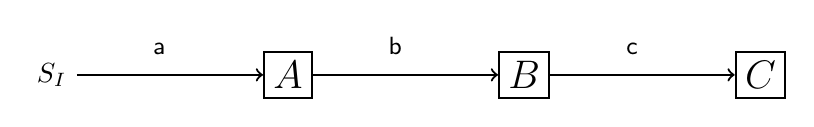
\begin{tikzpicture}[->,auto,node distance=3cm,
			thick,main node/.style={circle,draw,font=\sffamily\Large\bfseries},
			square node/.style={rectangle,draw,font=\sffamily\Large\bfseries}]
			
			\node[] (Invis) [] {$S_I$};
			\node[square node] (A) [right of=Invis] {$A$};
			\node[square node] (B) [right of=A] {$B$};
			\node[square node] (C) [right of=B] {$C$};
			
			
			\path[every node/.style={font=\sffamily\small}]
			(Invis) edge node [left, label=a] {} (A)
			(A) edge node [left, label=b] {} (B)
			(B) edge node [left, label=c] {} (C);
			\end{tikzpicture}		
		}
	\end{figure}
	
	The only decomposition for this problem results in the set of un-ordered actions $\{A, B, C\}$.
	If we consider that for the $3!$ linearizations of this set, the only executable one is $A, B, C$. This is impossible to achieve by linearized methods, since ordering either AB before C or C before AB will exclude the solution. 
	Even if we were to produce $k!$ methods for each partially ordered method with $k$ unordered sub-tasks, we would not be able to preserve any solution for this problem.
	
	This proves that the algorithm can remove all solutions, so Algorithm~\ref{alg:Algorithm1} is not complete. Note that incompleteness already follows from complexity theory as it's theoretically impossible to turn an arbitrary undecidable problem into a decidable one.
	Specifically, solutions that require interleaving of sub-tasks will not be preserved, as the example above demonstrates.
	
\end{proof}


We will now see that our algorithm preserves at least one solution as long as Algorithm~\ref{alg:Algorithm1} does not have to break cycles.
\begin{theorem}\label{thm:SpecialCase}
	Given a POHTN planning problem $P$ and TOHTN problem
	$P'$ obtained from $P$ by using Algorithm~\ref{alg:Algorithm1}, if Algorithm~\ref{alg:Algorithm1} did not have to
	cycle-break, then if the solution set of $P$ is non-empty then the solution set of $P'$ will be non-empty as well.
\end{theorem}
\begin{proof}
	Assume that there exists a solution in the PO domain. By using the same decomposition sequence in the linearized domain, we can produce the same set of actions as in the PO solution, but with a linearization of the actions decided by the linearized domain. Assume this sequence is $(a_0, a_1, ..., a_n)$. We then prove by induction over the sequence $(a_0, a_1, ..., a_n)$ that it is executable.
	If $(a_0, a_1, ..., a_n)$ is not executable, that means there exists some action $a_k,  0 < k < n$ that is not executable in the corresponding state. The action $a_k$ could only be non-executable, if one or more of its preconditions was not met. Assume one of these unmet preconditions is for existence of the state variable $A$.
	The action $a_k$ must be executable in some linearization of $\{a_0, ..., a_n\}$, as we assumed it was a PO solution. So there must exist an action $a_i$, $0 < i < n$, that will add A. Actions $a_0$ and $a_k$ must have a shared parent p in a Task Decomposition Tree. So p has subtasks $t_0$ and $t_k$ that are parents of $a_0$ and $a_k$ respectively. 
	
	The linearization of this method would have drawn an ordering $(t_i, t_k)$ due to the way the algorithm defines $prec^{*}, add^{*}$ etc. We are assuming that all methods linearized without conflict, so $(t_i, t_k)$ should not be required. This safely enforces $(a_k, a_0)$ ordering in the final TO plan, meaning $a_0$ is not the first action in the resulting total order imposed by the algorithm. In other words, if $a_k$’s precondition could be met by any action $a_i$, $a_i$ would be ordered in front of it. 
	
	If $a_i$ does not exist then $a_k$ can never be executed for any linearization of $\{a_0, ...a_n\}$, contradicting the assumption that this was a PO solution. Since each action in the solution is executable, the entire sequence is executable linearization of actions produced by decomposition of initial task, i.e.\ the solution.
\end{proof}

There are several levels of \enquote{completeness} possible. 
%\begin{enumerate}
\begin{compactitem}
	\item all solutions remain 
	\item at least one solution remains 
	\item all optimal solutions remain
	\item at least one optimal solution remains 	
\end{compactitem}
%\end{enumerate}
Given what's proven in Theorem~\ref{thm:notCompleteness} and \ref{thm:SpecialCase}, Algorithm~\ref{alg:Algorithm1} guarantees at least one solution remains, if no cycle-breaking is needed. If cycle-breaking is needed, Algorithm~\ref{alg:Algorithm1} makes no completeness guarantees at all -- it may remove all possible solutions. Finally, Algorithm~\ref{alg:Algorithm1} makes no decisions on any metric of optimality, so obviously cannot guarantee completeness that any optimal solutions remain.



\begin{theorem}\label{thm:newClass}
	For any problem $P$ that satisfies the criterion for linearization without cycle-breaking, the problem $P'$ obtained from applying the algorithm to $P$ forms a new class of decidable problems.
\end{theorem}
\begin{proof}
	A problem $P'$ obtained from applying Algorithm~\ref{alg:Algorithm1} to any arbitrary $P$ is a totally ordered problem, which are known to be decidable, as proven by \cite{Alford2015TightHTNBounds}.  
\end{proof}



\begin{theorem}\label{thm:Propositions}
	For any problem $P$ that satisfies the criterion for linearization without cycle-breaking, let the problem $P'$ be obtained from applying the algorithm to $P$. Let a decomposition of $P'$ be $D'$, and let the same decomposition of $P$ be $D$. Then if there exists any linearization of $D$ such that state variable $a$ can be true after execution of $D$, then $a$ will be true after execution of $D'$.
	
	In other words, Algorithm~\ref{alg:Algorithm1} finds the linearization that preserves $a$, for any state variable $a$, so long as one exists.
\end{theorem}
\begin{proof}
	\begin{figure}[h]
		\caption{Minimum requirement for loop}	
		\scalebox{0.8}{	\begin{subfigure}{6.5cm} 
				\begin{tikzpicture}[->,auto,node distance=1.5cm,
				thick,main node/.style={circle,draw,font=\sffamily\Large\bfseries},
				square node/.style={rectangle,draw,font=\sffamily\Large\bfseries}]
				
				\action{A1}{MinExampleA1,
					width  = 2.5em, 
					height = 2.5em, 
					pre length = 2em,
					eff length = 2em
				};			
				
				\action{A2}{MinExampleA2,
					width  = 2.5em, 
					height = 2.5em, 
					pre length = 2em,
					eff length = 2em,
					body = {right = 5em of A1} 
				};			
				
				\path[every node/.style={font=\sffamily\small}]
				(A1) edge[dashed, bend left] node [above] {} (A2)
				(A2) edge[dashed, bend left] node [above] {} (A1);
				\end{tikzpicture}
			\end{subfigure}	
		}	\scalebox{0.8}{	
			\begin{subfigure}{6.5cm}	
				\begin{tikzpicture}[->,auto,node distance=1.5cm,
				thick,main node/.style={circle,draw,font=\sffamily\Large\bfseries},
				square node/.style={rectangle,draw,font=\sffamily\Large\bfseries}]
				
				\action{A1}{MinExampleA3,
					width  = 2.5em, 
					height = 2.5em, 
					pre length = 2em,
					eff length = 2em
				};			
				
				\action{A2}{MinExampleA4,
					width  = 2.5em, 
					height = 2.5em, 
					pre length = 2em,
					eff length = 2em,
					body = {right = 5em of A1} 
				};			
				
				\path[every node/.style={font=\sffamily\small}]
				(A1) edge[dashed, bend left] node [above] {} (A2)
				(A2) edge[dashed, bend left] node [above] {} (A1);
				\end{tikzpicture}
			\end{subfigure}	
		}
		\scalebox{0.8}{
			\begin{subfigure}{6.5cm} 
				\begin{tikzpicture}[->,auto,node distance=1.5cm,
				thick,main node/.style={circle,draw,font=\sffamily\Large\bfseries},
				square node/.style={rectangle,draw,font=\sffamily\Large\bfseries}]
				
				\action{A1}{MinExampleA11,
					width  = 2.5em, 
					height = 2.5em, 
					pre length = 2em,
					eff length = 2em
				};			
				
				\action{A2}{MinExampleA12,
					width  = 2.5em, 
					height = 2.5em, 
					pre length = 2em,
					eff length = 2em,
					body = {right = 5em of A1} 
				};		
				
				\action{A3}{MinExampleA13,
					width  = 2.5em, 
					height = 2.5em, 
					pre length = 2em,
					eff length = 2em,
					body = {right = 5em of A2} 
				};			
				
				\path[every node/.style={font=\sffamily\small}]
				(A1) edge[dashed, bend left] node [above] {} (A2)
				(A2) edge[dashed, bend left] node [above] {} (A3)
				(A3) edge[dashed, bend left] node [above] {} (A1);
				\end{tikzpicture}
			\end{subfigure}	
		}
	\end{figure}
	
	Suppose for a given method, for any proposition $a$, $a \in \Pre(t)$ $a \in \Del(t')$ and $a \in \Add(t'')$, where $t, t', t''$ are sub-tasks. It's impossible for a task to have well-defined behaviour with both $\Del$ and $\Add$ for the same state variable. So it cannot be $t=t'=t''$. It can only be one task has $a \in \Pre, \Add$ and another $a \in \Del$, or one task has $a \in \Pre, a \in \Del$ and another has $a \in \Add$. The final option is $t t', t''$ are distinct. All options are shown in  as shown in the Figure~\ref{thm:Propositions}. Due to the rules of Algorithm~\ref{alg:Algorithm1}, all options result in a loop.	
	
	The remaining options then are to have just one or two of $\Pre, \Add$, or $\Del$- this can generate at most one edge, and so any loops that occur in the final graph must be from other interactions between other state variables.
	
	If only one, any linearization results in the same result for $p$ in the final state. If only two, the ordering is $\Pre, \Del$, resulting in unavoidable deletion, or $\Del, \Add$, resulting in preservation of $p$, or $\Add, \Pre$, resulting in preservation of $p$.
	
\end{proof}


%\begin{theorem}
%	Cycle-breaking is not guaranteed to eliminate solutions.
%\end{theorem}
%\begin{proof}
%	As per proposition 2.1 and 2.2, not all of the preconditions and effects are always needed. Suppose the initial task network consisted of 2 sub-tasks, $t_1, t_2$. If $t_2$ can decompose into an action $a_1$ such that $add(a_1) = A$, and an action $a_2$ such that $del(a_2) = A$,
%	and $t_1$ can decompose into an action $a_3$ with $prec(a_3) = A$
%	$t_2 = {add A, del A}$ and $t_1 = {prec A}$. The rules $\{(add A, prec A), (prec A, del A))\}$ of Algorthm 1
%	require orderings $\{(t_2, t_2), (t_2, t_1), (t_1, t_2)\}$, i.e.
%	Despite a cycle break being needed, this is obviously a solvable problem. Order $t_2$ before $t_1$ for this method.
%	Then when solving decompose $t_2$ to $a_1$ and $t_1$ to $a_3$. This creates a solution. Therefore, it is possible for the algorithm to preserve solutions despite needing cycle-breaking.
%\end{proof}

%%%%  
%\begin{theorem}
%	Given a POHTN planning problem $P = (F, T_P, T_C, \delta, M)$, for a given method $m \in M$, if some task $t \in T_P \cup T_C$ does not have an ordering applied to it by the graph $G$ built in lines 4-11 of Algorithm 1, 
%	then for the TOHTN problem $P'$ obtained from $P$ by using Algorithm 1,
%	the ordering of $t$ will not affect the executability of the final solution.
%	Given a method with all such tasks will cause the solution set of $P$ to equal the solution set of $P'$
%	Or in other words, if a linearization exists at all, it's possible to remove some edges from $G$ in Algorithm 1 to obtain it.
%\end{theorem}
%\begin{proof}
%	Assume that some pair of tasks $t_1, t_2$, Algorithm 1 did not add an ordering between them based off their preconditions and effects. Assume also that the ordering $t_1, t_2$ is executable but $t_2,t_1$ is not, i.e.
%	it matters where they are executed relative to each other.  \newline  \newline
%	This implies that $t_2$ deletes some variable A $t_1$ relies on. But from the definition of Algorithm 1,
%	that would mean that an ordering $(t_1, t_2)$ was created, which contradicts the assumption that there is no ordering between them.
%	Therefore $(t_2, t_1)$ ordering must also be executable. \newline  \newline
%	Thus if some task t has no ordering from the algorithm, it can never matter where it is in relation to any other task.
%	The algorithm will not order it specifically when $(\forall t' \in m, \forall a \in prec(t). a \notin add(t') \land a \notin del(t'))
%	\land  (\forall t' \in m, \forall a \in add(t). a \notin prec(t') \land a \notin del(t')) 
%	\land  (\forall t' \in m, \forall a \in del(t). a \notin add(t') \land a \notin prec(t'))$
%	In other words, the variables that affect t, do not affect other tasks in that method.
%\end{proof}


% \todo{the environments 'definition', 'lemma', 'proposition', 'corollary', 'remark', and 'example' are defined in the LLNCS documentclass as well.}


